%%%%%%%%%%%%%%%%%%%%%%%%%%%%%%%%%%%%%%%%%
% Jacobs Landscape Poster
% LaTeX Template
% Version 1.1 (14/06/14)
%
% Created by:
% Computational Physics and Biophysics Group, Jacobs University
% https://teamwork.jacobs-university.de:8443/confluence/display/CoPandBiG/LaTeX+Poster
% 
% Further modified by:
% Nathaniel Johnston (nathaniel@njohnston.ca)
%
% This template has been downloaded from:
% http://www.LaTeXTemplates.com
%
% License:
% CC BY-NC-SA 3.0 (http://creativecommons.org/licenses/by-nc-sa/3.0/)
%
%%%%%%%%%%%%%%%%%%%%%%%%%%%%%%%%%%%%%%%%%

%----------------------------------------------------------------------------------------
% PACKAGES AND OTHER DOCUMENT CONFIGURATIONS
%----------------------------------------------------------------------------------------

\documentclass[final]{beamer}

\usepackage{amsmath}
\usepackage[framemethod=TikZ]{mdframed}
\usepackage[scale=1.24]{beamerposter} % Use the beamerposter package for laying out the poster

\usetheme{confposter} % Use the confposter theme supplied with this template

\setbeamercolor{block title}        {fg=DarkRed,bg=white} % Colors of the block titles
\setbeamercolor{block body}         {fg=black,bg=white} % Colors of the body of blocks
\setbeamercolor{block alerted title}{fg=white,bg=Cardinal} % Colors of the highlighted block titles
\setbeamercolor{block alerted body} {fg=black,bg=Sandstone20} % Colors of the body of highlighted blocks
\setbeamercolor{item}               {fg=black}
\setbeamercolor{item project}       {fg=black}
% Many more colors are available for use in beamerthemeconfposter.sty

%-----------------------------------------------------------
% Define the column widths and overall poster size
% To set effective sepwid, onecolwid and twocolwid values, first choose how many columns you want and how much separation you want between columns
% In this template, the separation width chosen is 0.024 of the paper width and a 4-column layout
% onecolwid should therefore be (1-(# of columns+1)*sepwid)/# of columns e.g. (1-(4+1)*0.024)/4 = 0.22
% Set twocolwid to be (2*onecolwid)+sepwid = 0.464
% Set threecolwid to be (3*onecolwid)+2*sepwid = 0.708

\newlength{\sepwid}
\newlength{\onecolwid}
\newlength{\twocolwid}
\newlength{\threecolwid}
\setlength{\paperwidth}{48in} % A0 width: 46.8in
\setlength{\paperheight}{36in} % A0 height: 33.1in
\setlength{\sepwid}{0.024\paperwidth} % Separation width (white space) between columns
\setlength{\onecolwid}{0.22\paperwidth} % Width of one column
\setlength{\twocolwid}{0.464\paperwidth} % Width of two columns
\setlength{\threecolwid}{0.708\paperwidth} % Width of three columns
\setlength{\topmargin}{-0.5in} % Reduce the top margin size
%-----------------------------------------------------------

\usepackage{graphicx}  % Required for including images

\usepackage{booktabs} % Top and bottom rules for tables
\usepackage[backend=biber,style=alphabetic,citestyle=authoryear]{biblatex}
\addbibresource{presentation_bib.bib}
\usepackage{framed}
\usepackage{multicol}

%----------------------------------------------------------------------------------------
% TITLE SECTION 
%----------------------------------------------------------------------------------------

\title{Fine-Grained Opinion Tagging Using Deep Recurrent Nets with GRUs} % Poster title

\author{Alex Adamson and Deger Turan} % Author(s)

\institute{Stanford University} % Institution(s)

%----------------------------------------------------------------------------------------

\begin{document}

\nocite{*}

\makeatletter
\renewcommand{\overset}[2]{\ensuremath{\mathop{\kern\z@\mbox{#2}}\limits^{\mbox{\scriptsize #1}}}}
\renewcommand{\underset}[2]{\ensuremath{\mathop{\kern\z@\mbox{#2}}\limits_{\mbox{\scriptsize #1}}}}
\makeatother

\addtobeamertemplate{block end}{}{\vspace*{2ex}} % White space under blocks
\addtobeamertemplate{block alerted end}{}{\vspace*{2ex}} % White space under highlighted (alert) blocks

\setlength{\belowcaptionskip}{2ex} % White space under figures
\setlength\belowdisplayshortskip{2ex} % White space under equations

\begin{frame}[t] % The whole poster is enclosed in one beamer frame

\begin{columns}[t] % The whole poster consists of three major columns, the second of which is split into two columns twice - the [t] option aligns each column's content to the top

\begin{column}{\sepwid}\end{column} % Empty spacer column

\begin{column}{\onecolwid} % The first column

%----------------------------------------------------------------------------------------
% OBJECTIVES
%----------------------------------------------------------------------------------------

\begin{alertblock}{Objectives}

Lorem ipsum dolor sit amet, consectetur, nunc tellus pulvinar tortor, commodo eleifend risus arcu sed odio:
\begin{itemize}
\item Mollis dignissim, magna augue tincidunt dolor, interdum vestibulum urna
\item Sed aliquet luctus lectus, eget aliquet leo ullamcorper consequat. Vivamus eros sem, iaculis ut euismod non, sollicitudin vel orci.
\end{itemize}

\end{alertblock}

%----------------------------------------------------------------------------------------
% INTRODUCTION
%----------------------------------------------------------------------------------------

\begin{block}{Introduction}

The fine-grained opinion mining task seeks to, given textual input, find the opinions expressed therein, their intensity and other properties such as their holder and their target. In our work, we focus on the task of tagging attitudes, attitude holders and attitude targets contained in a given sentence. In particular, we first explore the fitness of a deep bidirectional recurrent network for this task using the work described in \cite{irsoy2014opinion} and then attempt to extend it by using gated recurrent units (\cite{DBLP:journals/corr/ChungGCB15}) instead of vanilla ReLU units.

\end{block}

%------------------------------------------------

\begin{figure}
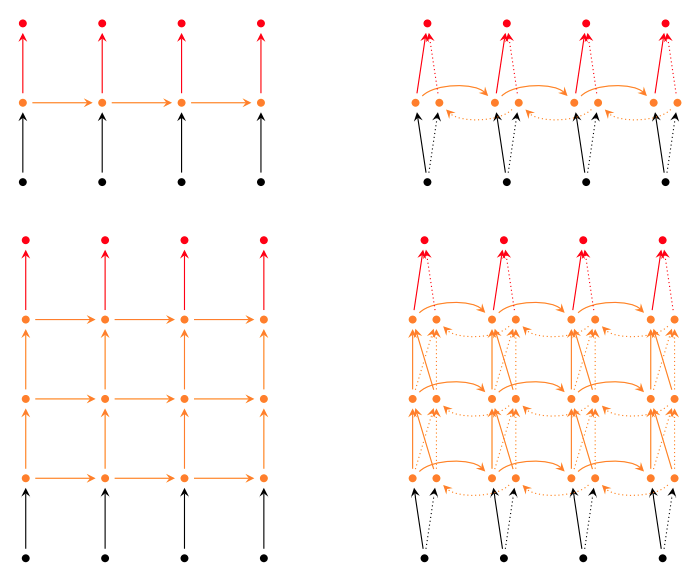
\includegraphics[width=0.8\linewidth]{bidrnn-irsoy.png}
\caption{Taken from \cite{irsoy2014opinion}: Clockwise from top left: single-layer recurrent neural network, single-layer bidirectional recurrent neural network, deep bidirectional recurrent neural network, deep recurrent neural neural network. Forward layers are denoted with solid lines and backward layers are denoted with dotted lines. Input layers, hidden layers and output layers are shown in black, orange and red respectively.}
\label{bidrnn-fig}
\end{figure}

%----------------------------------------------------------------------------------------

\end{column} % End of the first column

\begin{column}{\sepwid}\end{column} % Empty spacer column

\begin{column}{\twocolwid} % Begin a column which is two columns wide (column 2)

% \begin{columns}[t,totalwidth=\twocolwid] % Split up the two columns wide column

% \end{columns} % End of the split of column 2 - any content after this will now take up 2 columns width

\begin{column}{\twocolwid}\vspace{-.6in} % The first column within column 2 (column 2.1)

%----------------------------------------------------------------------------------------
% MATERIALS
%----------------------------------------------------------------------------------------

\begin{block}{Dataset}

We use the MPQA 2.0 dataset (\cite{wiebe2005annotating}). The dataset consists of 15737 sentences drawn from the world English-language press. Each sentence is tagged by a trained human for features such as attitudes, attitude targets, attitude holders (agents), objective speech events, and various subjective statements.

\begin{alertblock}{Example annotation}
[\textbf{"The quickest }\underset{target}{\textbf{[defeat of Tsvangirai and his MDC lot]}} \underset{attitude}{\textbf{would come if}} \textbf{they chose the path of violence,"]} \underset{agent}{\textbf{[an analyst]}} who spoke on condition of anonymity said.
\end{alertblock}

\end{block}

%----------------------------------------------------------------------------------------

\end{column} % End of column 2.1

\begin{column}{\twocolwid}\vspace{-.6in} % The second column within column 2 (column 2.2)

%----------------------------------------------------------------------------------------
% METHODS
%----------------------------------------------------------------------------------------

\begin{block}{Methods}

The models we constructed and evaluated include a softmax regression baseline, the deep bidirectional recurrent network described and implemented by Ozan Irsoy (\cite{irsoy2014opinion}), and an extension of Irsoy's network that used gated recurrent units instead of ReLU nonlinearities. In particular, whereas Irsoy's model uses the following definition for his interior hidden units

\begin{framed}
\begin{align}
  \overrightarrow{h}_t^{(i)} &= f(\underrightarrow{\overrightarrow{W}}^{(i)} \overrightarrow{h}_t^{(i-1)} + \underleftarrow{\overrightarrow{W}}^{(i)} \overleftarrow{h}_t^{(i-1)} + \overrightarrow{V}^{(i)} \overrightarrow{h}_{t-1}^{(i)} + \overrightarrow{b}^{(i)}) \\
  \overleftarrow{h}_t^{(i)} &= f(\underrightarrow{\overleftarrow{W}}^{(i)} \overrightarrow{h}_t^{(i-1)} + \underleftarrow{\overleftarrow{W}}^{(i)} \overleftarrow{h}_t^{(i-1)} + \overleftarrow{V}^{(i)} \overleftarrow{h}_{t=1}^{(i)} + \overleftarrow{b}^{(i)})
\end{align}
\end{framed}

the GRU model uses

\begin{framed}
\begin{align}
  \overrightarrow{z}_t^{(i)} &= f_2(\underrightarrow{\overrightarrow{Wz}}^{(i)} \overrightarrow{h}_t^{(i-1)} + \underleftarrow{\overrightarrow{Wz}}^{(i)} \overleftarrow{h}_t^{(i-1)} + \overrightarrow{Vz}^{(i)} \overrightarrow{h}_{t-1}^{(i)}) \\
  \overrightarrow{r}_t^{(i)} &= f_2(\underrightarrow{\overrightarrow{Wr}}^{(i)} \overrightarrow{h}_t^{(i-1)} + \underleftarrow{\overrightarrow{Wr}}^{(i)} \overleftarrow{h}_t^{(i-1)} + \overrightarrow{Vr}^{(i)} \overrightarrow{h}_{t-1}^{(i)}) \\
  \widetilde{\overrightarrow{h}}_t^{(i)} &= f(\underrightarrow{\overrightarrow{W}}^{(i)} \overrightarrow{h}_t^{(i-1)} + \underleftarrow{\overrightarrow{W}}^{(i)} \overleftarrow{h}_t^{(i-1)} + \overrightarrow{r}_t^{(i)} \circ \overrightarrow{V}^{(i)} \overrightarrow{h}_{t-1}^{(i)}) \\
  \overrightarrow{h}_t^{(i)} &= \overrightarrow{z}_t^{(i)} \circ \overrightarrow{h}_{t-1}^{(i)} + (1 - \overrightarrow{z}_t^{(i)}) \circ \widetilde{\overrightarrow{h}}_t^{(i)}
\end{align}
and analogously for the right-to-left units.
\end{framed}

Training the models proved to be difficult. Using a standard supervised error signal and without introducing any weighting to particular kinds of errors, both recurrent networks would converge to something that looked like the prior when trained using minibatch gradient descent.

In order to make the models converge to something meaningful, we took the following steps:
\begin{itemize}
\item Introducing a linear transformation of the error signal from the output layer to the error vector passed down by each hidden layer
\item Reducing penalties incurred by misclassifying tokens as non-null by multiplying by a constant factor
\item Using a momentum rate when performing gradient descent
\end{itemize}
With these modifications, the models would generally converge without significant oscillatory behavior.
\end{block}


%----------------------------------------------------------------------------------------

\end{column} % End of column 2.2

%----------------------------------------------------------------------------------------
% IMPORTANT RESULT
%----------------------------------------------------------------------------------------

\begin{alertblock}{Important Result}

Lorem ipsum dolor \textbf{sit amet}, consectetur adipiscing elit. Sed commodo molestie porta. Sed ultrices scelerisque sapien ac commodo. Donec ut volutpat elit.

\end{alertblock} 

\end{column} % End of the second column

\begin{column}{\sepwid}\end{column} % Empty spacer column

\begin{column}{\onecolwid} % The third column

%----------------------------------------------------------------------------------------
% CONCLUSION
%----------------------------------------------------------------------------------------

\begin{block}{Results}

\begin{tabular}{r | l r | c c | c c | c c |} \cline{2-9}
                 & Model & $|h|$ & \multicolumn{2}{|c|}{Precision} & \multicolumn{2}{|c|}{Recall} & \multicolumn{2}{|c|}{F1} \\ \cline{2-9}
                 &       &       & Prop. & Bin.  & Prop. & Bin.  & Prop. & Bin. \\ \cline{2-9}
\small{Agent}    & DRNN  & 25    & 0.653 & 0.675 & 0.707 & 0.746 & 0.679 & 0.709 \\
                 & GRU   & 25    & 0.632 & 0.661 & 0.675 & 0.722 & 0.653 & 0.690  \\ \cline{2-9}
\small{Attitude} & DRNN  & 25    & 0.276 & 0.344 & 0.625 & 0.733 & 0.383 & 0.468 \\
                 & GRU   & 25    & 0.291 & 0.360 & 0.575 & 0.672 & 0.386 & 0.469  \\ \cline{2-9}
\small{Target}   & DRNN  & 25    & 0.243 & 0.280 & 0.398 & 0.514 & 0.302 & 0.362 \\
                 & GRU   & 25    & 0.266 & 0.320 & 0.343 & 0.447 & 0.300 & 0.373  \\ \cline{2-9}
\end{tabular}

\end{block}

%----------------------------------------------------------------------------------------
% REFERENCES
%----------------------------------------------------------------------------------------

\begin{block}{References}

\printbibliography

\end{block}

%----------------------------------------------------------------------------------------
% ACKNOWLEDGEMENTS
%----------------------------------------------------------------------------------------

\setbeamercolor{block title}{fg=red,bg=white} % Change the block title color

\begin{block}{Acknowledgements}

\small{\rmfamily{Nam mollis tristique neque eu luctus. Suspendisse rutrum congue nisi sed convallis. Aenean id neque dolor. Pellentesque habitant morbi tristique senectus et netus et malesuada fames ac turpis egestas.}} \\

\end{block}

%----------------------------------------------------------------------------------------
% CONTACT INFORMATION
%----------------------------------------------------------------------------------------

\setbeamercolor{block alerted title}{fg=black,bg=norange} % Change the alert block title colors
\setbeamercolor{block alerted body}{fg=black,bg=white} % Change the alert block body colors

\begin{alertblock}{Contact Information}

\begin{itemize}
\item Web: \href{http://www.university.edu/smithlab}{http://www.university.edu/smithlab}
\item Email: \href{mailto:john@smith.com}{john@smith.com}
\item Phone: +1 (000) 111 1111
\end{itemize}

\end{alertblock}

\begin{center}
\begin{tabular}{ccc}

\includegraphics[width=0.4\linewidth]{logo.png} & \hfill & 
\includegraphics[width=0.4\linewidth]{logo.png}
\end{tabular}
\end{center}

%----------------------------------------------------------------------------------------

\end{column} % End of the third column

\end{columns} % End of all the columns in the poster

\end{frame} % End of the enclosing frame

\end{document}
